\chapter{Lexing with regular expression}
\label{chap:lexing_regular_expr}

\section{Importance of Lexing}
    \subsection{Whitespace Handling}
        This chapter will show why lexing is important in addition to parsing. A
        simple example is whitespace (WS) handling. If we look at the grammar we
        have defined before (N, P, S) the expression " 1 + 1 " is not accepted
        because of whitespace. In order to have WS accepted we can use the
        following rule : $S ::= S '+' WS* P | S '-' WS* P | P$  with WS being
        space, $\backslash$t or $\backslash$n but it is not nice and can quickly
        become a mess. A nicer approach would be to define WS as before and to
        define new rules for operators like $PLUS ::= '+' WS*$.
    \subsection{CFG limitation}
        As we have seen before CFG does not allow reserved work like if.
    \subsection{Performances}
        If we don't use lexing, we need to work on each character, using a lexer
        we can build a token tree which can be ~20 smaller. This is especially
        true if there are fixed overheads (combinators). It is typically
        developed as a loop with switch statement. It is simple enough that we
        can write it by hand or even better generate it (regular expressions)!
\section{Lexers with RE}
    The idea is that we want to match a prefix of the (remainder of) input that
    matches the RE. There are two types of RE flavors : 
    \begin{itemize}
        \item Standard (equivalent to regular grammars) : can be matched in
        $\mathcal{O}(n)$ (n=input size)
        \item Language specific (Perl-Compatible Regular Expression) : often in
        $\mathcal{O}(n)$ but some features can make it exponential (even without
        using them). E.g : backreferencing (capture something we have match and
        try to match it again).
    \end{itemize}

    \newpage
    Some experiment on this subject have been made which show the time needed by
    both techniques to match some rules. As we can see on the next figure the
    difference is huge. Note that, the y axes is not the same, with PCRE we're
    speaking in seconds while in the other approach we are on $\mu$s which is
    way smaller!
    \begin{figure}[H]
         \centering
         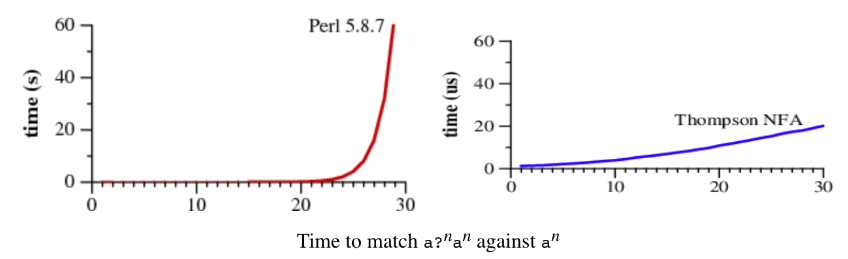
\includegraphics[scale=0.4]{comparison.png}
         \caption{Regular vs PCRE}
         \label{fig:regu_vs_pcre}
    \end{figure}

    However we can ask ourself if this experiment is really realistic. As we
    have seen, it \textit{can} be exponential in some case but are these case
    something that can really happen? This question is not so easy to answer if
    we make some research (Pr. did) we can maybe find one grammar example that
    is both useful and exponential.

    Let's now image that matching a RE is done in $\mathcal{O}(n)$, what is the
    complexity of lexing? It is $\mathcal{O}(n^2)$! Why ? Because in the worst
    case we would need to scan to the end of the input (n) for each token. An
    example would be : $(a | a*x)$ with $a^n$ as input. This is a contrived
    example which is not a problem in practice! This is also a nice example of
    theory vs practice.

\section{Building the DFA}
    We have seen before that regular grammars can be recognized by a
    Deterministic Finite Automaton. First let's look at the DFA for rule $Tokens
    ::= [0-9]+ | [a-z] | "if"$. The resulting automaton is this one :
    \begin{figure}[H]
         \centering
         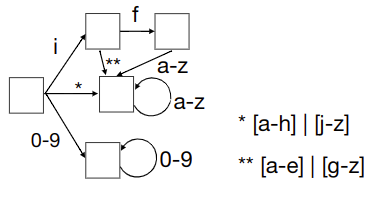
\includegraphics[scale=0.4]{Automaton.png}
         \caption{DFA example}
         \label{fig:dfa_ex}
    \end{figure}

    In order to build the DFA, we first need to translate the regular expression
    to a NFA (Non-deterministic Finite Automaton). Then we have two options :
    \begin{enumerate}
        \item \begin{itemize}
            \item Transform the NFA into a DFA
            \item Minimize the DFA
        \end{itemize}
        \item \begin{itemize}
            \item Simulate DFA with a NFA
            \item Exactly the same thing, but lazily
        \end{itemize}
    \end{enumerate}
\newpage
\section{NFA}
    First of all let's see an example of NFA, the left part is showing the NFA
    whereas the right part is the equivalent DFA. As we can see, the difference
    is that in NFA we can have multiple transition that use the same letter. 
    \begin{figure}[H]
         \centering
         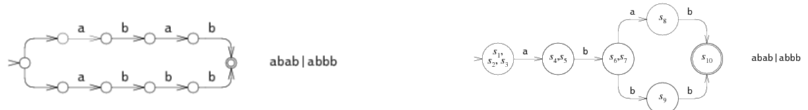
\includegraphics[scale=0.5]{NFA_VS_DFA}
         \caption{NFA example}
         \label{fig:nfa_ex}
    \end{figure}
    If we try to match a sequence in a NFA, we have two ways : 
    \begin{itemize}
        \item Keeping a single pointer that rollback at the beginning if the
        match failed
        \item Keeping multiple pointer that go in parallel.
    \end{itemize}

    In DFA the complexity is $\mathcal{O}(n)$ well, in fact it's more
    $\mathcal{O}(nm^2)$ (at least in theory) where m = number of states and
    represent the possibility where every state is connected to each other. In
    practice, NFA use repeated work and more complex data structures. That, plus
    the fact that DFA are pure $\mathcal{O}(n)$ make them more usable in
    practice.

    \subsection{From regex to NFA}
        Here is the list of regex when applied with NFA : 
        \begin{figure}[H]
             \centering
             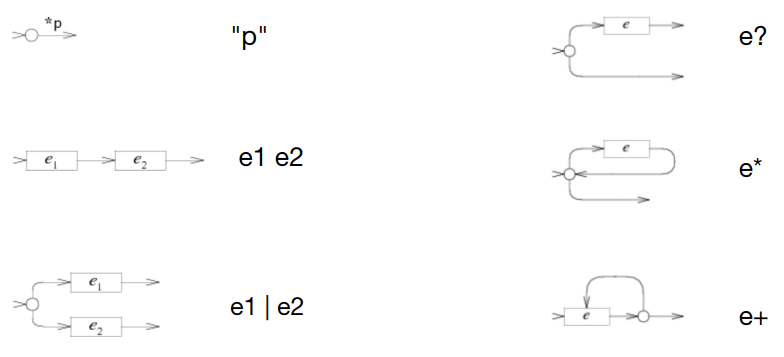
\includegraphics[scale=0.4]{regex_to_nfa.png}
             \caption{Regex to NFA}
             \label{fig:regex_nfa}
        \end{figure}
        Note that $e_1, e_2$ are complete automaton that are plugged. Also if we
        don't have starting point (like in $e_1 e_2$) it means that the starting
        state of $e_1$ become the starting state of the whole sequence.

        Empty transitions are very useful in order to keep the number of
        transition manageable. Without them, every state would need to be link
        together (so, for 2 choice of 3 letters, 12 transitions, 9 with empty
        transitions.)

\section{Powerset construction}
    Powerset construction is a technique that allow us to transform a NFA to
    DFA. It is quiet simple, we take concurrent equivalent states and merge them
    into a single one in the DFA. Figure \ref{fig:nfa_ex} show the 
\section{Minimization of DFA}
    When we "translate" a NFA to a DFA we may end up with an increasing size!
    e.g a NFA of size n, may lead to an DFA of size $2^n$. We cannot do anything
    for that expect to minimize a little the DFA.

    These two algorithms are classical ones in compilers classes.

\section{DFA simulation}
    It use the Thompson's algorithm : 
    \begin{itemize}
        \item Run the NFA by maintaining a list of states
        \item Build the DFA by treating the list of states as a single DFA
        state.
        \item Need to be able to lookup a DFA state from a list of NFA state.
    \end{itemize}

    This approach is typically slower as we do the work while lexing. However,
    the main advantage is that we only build DFA node that we need!